\documentclass[11pt]{article}

% ============================================================
%  preamble.tex  --  packages, styling, custom environments
% ============================================================

% ---------- page ----------
\usepackage[a4paper,margin=1in,marginparwidth=1.1in,headheight=14pt]{geometry}

% ---------- math ----------
\usepackage{amsmath,amssymb,amsthm}
\usepackage{mathtools}
\usepackage{bm}

% ---------- fonts ----------
\usepackage[T1]{fontenc}
\usepackage{newpxtext}
\usepackage{newpxmath}
\usepackage[scaled=0.90]{helvet}   % sans face for box titles / headers
% expansion=false: some newpx faces here are not scalable, and font expansion
% is a fatal error with those. Protrusion still works and does most of the good.
\usepackage[expansion=false]{microtype}

% ---------- graphics / tables ----------
\usepackage{graphicx}
\usepackage{booktabs}
\usepackage{tabularx}
\usepackage{enumitem}
\usepackage{caption}
\usepackage{subcaption}
\usepackage{tikz}
\usetikzlibrary{arrows.meta,positioning,calc,patterns,
                decorations.pathmorphing,decorations.pathreplacing}
\usepackage{pgfplots}
\pgfplotsset{compat=1.18}

% ---------- headers ----------
\usepackage{fancyhdr}
\pagestyle{fancy}
\fancyhf{}
\fancyhead[L]{\small\sffamily\nouppercase{\leftmark}}
\fancyhead[R]{\small\sffamily\thepage}
\renewcommand{\headrulewidth}{0.4pt}

% ---------- colors ----------
\usepackage{xcolor}
\definecolor{IntFrame}{HTML}{1F6F8B}   % intuition   - teal
\definecolor{IntBack} {HTML}{EAF3F6}
\definecolor{DicFrame}{HTML}{6B4E9E}   % dictionary  - purple
\definecolor{DicBack} {HTML}{F2EEF9}
\definecolor{PitFrame}{HTML}{B23A3A}   % pitfall     - red
\definecolor{PitBack} {HTML}{FBEDED}
\definecolor{RecFrame}{HTML}{7A7A7A}   % recall      - grey
\definecolor{RecBack} {HTML}{F4F4F4}
\definecolor{MEFrame} {HTML}{2E7D4F}   % worked ME   - green
\definecolor{MEBack}  {HTML}{EBF5EF}
\definecolor{RoadFrame}{HTML}{B5651D}   % roadmap     - burnt orange
\definecolor{RoadBack} {HTML}{FDF3E9}
\definecolor{LinkCol} {HTML}{16506B}

% ---------- links ----------
\usepackage{hyperref}
\hypersetup{
  colorlinks=true,
  linkcolor=LinkCol, citecolor=LinkCol, urlcolor=LinkCol,
  pdfborder={0 0 0}
}
\usepackage{xurl}

% ---------- theorem environments ----------
\theoremstyle{definition}
\newtheorem{definition}{Definition}[section]
\newtheorem{example}[definition]{Example}
\newtheorem{exercise}[definition]{Exercise}

\theoremstyle{plain}
\newtheorem{theorem}[definition]{Theorem}
\newtheorem{lemma}[definition]{Lemma}
\newtheorem{proposition}[definition]{Proposition}
\newtheorem{corollary}[definition]{Corollary}

\theoremstyle{remark}
\newtheorem{remark}[definition]{Remark}

% ---------- boxes ----------
\usepackage[most]{tcolorbox}
\tcbset{
  femboxbase/.style={
    enhanced, breakable, sharp corners=downhill,
    boxrule=0.8pt, left=8pt, right=8pt, top=6pt, bottom=6pt,
    fonttitle=\bfseries\sffamily\small,
    attach boxed title to top left={xshift=8pt, yshift=-\tcboxedtitleheight/2},
    boxed title style={sharp corners, boxrule=0pt, size=small},
    toptitle=2pt,
  }
}

% Intuition: the "why does this object exist / what is it really" box.
\NewTColorBox{intuition}{ o }{%
  femboxbase, colback=IntBack, colframe=IntFrame,
  coltitle=white, colbacktitle=IntFrame,
  title={Intuition\IfValueT{#1}{: #1}}
}

% Pitfall: the specific place ME students get derailed.
\NewTColorBox{pitfall}{ o }{%
  femboxbase, colback=PitBack, colframe=PitFrame,
  coltitle=white, colbacktitle=PitFrame,
  title={Where this trips people up\IfValueT{#1}{: #1}}
}

% Recall: prerequisite you were assumed to already have.
\NewTColorBox{recall}{ o }{%
  femboxbase, colback=RecBack, colframe=RecFrame,
  coltitle=white, colbacktitle=RecFrame,
  title={Recall\IfValueT{#1}{: #1}}
}

% Mechanics: the concrete engineering instance of the abstract statement.
\NewTColorBox{mechanics}{ o }{%
  femboxbase, colback=MEBack, colframe=MEFrame,
  coltitle=white, colbacktitle=MEFrame,
  title={In mechanics terms\IfValueT{#1}{: #1}}
}

% Roadmap: the bullet-point big picture, at the top of every lecture.
% The lecturer writes maybe half of what he says; this is the half that
% went missing -- what the lecture is for and what it buys you.
\NewTColorBox{roadmap}{ o }{%
  femboxbase, colback=RoadBack, colframe=RoadFrame,
  coltitle=white, colbacktitle=RoadFrame,
  title={The big picture\IfValueT{#1}{: #1}},
  after skip=14pt
}
\newlist{roadlist}{itemize}{1}
\setlist[roadlist]{label=\textcolor{RoadFrame}{\small$\blacktriangleright$},
  leftmargin=1.6em, topsep=4pt, itemsep=3.5pt, parsep=0pt}
% the one-line question the lecture answers, and the one-line payoff
\newcommand{\roadq}[1]{\noindent\textit{#1}}
\newcommand{\payoff}[1]{\par\smallskip\noindent
  \textbf{\color{RoadFrame}Use it for:}\ #1}

% Dictionary: two-column math <-> mechanics translation table.
\NewTColorBox{dictbox}{ o }{%
  femboxbase, colback=DicBack, colframe=DicFrame,
  coltitle=white, colbacktitle=DicFrame,
  title={Translation\IfValueT{#1}{: #1}}
}

% tabularx must see its whole body at once, so the rows are captured with
% environ's \BODY rather than split across a \newenvironment.
\usepackage{environ}
\NewEnviron{dictionary}[1][]{%
  \ifstrempty{#1}{\begin{dictbox}}{\begin{dictbox}[#1]}%
  \renewcommand{\arraystretch}{1.25}%
  \begin{tabularx}{\linewidth}{@{}>{\raggedright\arraybackslash}X@{\hspace{1em}}>{\raggedright\arraybackslash}X@{}}
  \toprule
  \textbf{Math department writes} & \textbf{You should hear}\\
  \midrule
  \BODY
  \bottomrule
  \end{tabularx}%
  \end{dictbox}%
}

% ---------- lecture heading ----------
\usepackage{titlesec}
\newcommand{\lecture}[3]{%
  \section[#1]{#1}%
  \noindent{\small\sffamily\color{RecFrame} #2 \hfill #3}\par
  \vspace{0.4em}\hrule\vspace{1em}%
}

% ---------- transcript switch ----------
% \transcripttrue in a master file  ->  suppress the added commentary,
% leaving only the transcribed lecture. Default: full annotated notes.
\newif\iftranscript
\transcriptfalse

% ---------- verdict marks ----------
\newcommand{\cmark}{\textcolor{MEFrame}{\ensuremath{\checkmark}}}
\newcommand{\xmark}{\textcolor{PitFrame}{\ensuremath{\times}}}

% ---------- open questions marker ----------
\newcommand{\todoq}[1]{%
  \par\noindent{\color{PitFrame}\sffamily\small$\blacktriangleright$ \textbf{Unclear in my notes:} #1}\par
}

\allowdisplaybreaks

% ============================================================
%  macros.tex  --  FEM notation shortcuts
% ============================================================

% ---------- sets ----------
\newcommand{\R}{\mathbb{R}}
\newcommand{\N}{\mathbb{N}}
\newcommand{\Z}{\mathbb{Z}}
\newcommand{\Om}{\Omega}
\newcommand{\dOm}{\partial\Omega}
\newcommand{\GD}{\Gamma_{\!D}}          % Dirichlet boundary
\newcommand{\GN}{\Gamma_{\!N}}          % Neumann boundary

% ---------- function spaces ----------
\newcommand{\Ltwo}[1][\Om]{L^{2}(#1)}
\newcommand{\Hs}[2][\Om]{H^{#2}(#1)}
\newcommand{\Hone}[1][\Om]{H^{1}(#1)}
\newcommand{\Honez}[1][\Om]{H^{1}_{0}(#1)}
\newcommand{\Ck}[2][\Om]{C^{#2}(#1)}
\newcommand{\Cinfz}[1][\Om]{C^{\infty}_{c}(#1)}
\newcommand{\Vsp}{V}                    % trial/test space
\newcommand{\Vh}{V_{h}}                 % discrete subspace

% ---------- solutions ----------
\newcommand{\uh}{u_{h}}
\newcommand{\vh}{v_{h}}
\newcommand{\eh}{e_{h}}
\newcommand{\Ih}{\mathcal{I}_{h}}       % interpolant
\newcommand{\Th}{\mathcal{T}_{h}}       % triangulation
\newcommand{\Kel}{K}                    % generic element
\newcommand{\Kref}{\widehat{K}}         % reference element

% ---------- operators ----------
\renewcommand{\div}{\operatorname{div}}
\newcommand{\grad}{\nabla}
\newcommand{\lap}{\Delta}
\newcommand{\dd}{\,\mathrm{d}}
\newcommand{\dx}{\dd x}
\newcommand{\ds}{\dd s}
\newcommand{\pd}[2]{\frac{\partial #1}{\partial #2}}
\newcommand{\nn}{\bm{n}}                % outward normal
\newcommand{\supp}{\operatorname{supp}}
\newcommand{\tr}{\operatorname{tr}}

% ---------- forms, norms, pairings ----------
\newcommand{\bl}[2]{a(#1,#2)}                            % bilinear form
\newcommand{\Lf}[1]{\ell(#1)}                            % linear functional
\DeclarePairedDelimiter{\abs}{\lvert}{\rvert}
\DeclarePairedDelimiter{\norm}{\lVert}{\rVert}
\newcommand{\Lnorm}[2][\Om]{\norm{#2}_{\Ltwo[#1]}}
\newcommand{\Hnorm}[2][\Om]{\norm{#2}_{\Hone[#1]}}
\newcommand{\Enorm}[1]{\vertiii{#1}}                     % energy norm
\newcommand{\vertiii}[1]{{\left\vert\kern-0.25ex\left\vert\kern-0.25ex\left\vert #1
  \right\vert\kern-0.25ex\right\vert\kern-0.25ex\right\vert}}
\newcommand{\ipL}[3][\Om]{\left(#2,#3\right)_{#1}}       % L2 inner product
\newcommand{\dual}[2]{\left\langle #1,#2\right\rangle}   % duality pairing

% ---------- discrete / matrix ----------
\newcommand{\Kmat}{\bm{K}}              % stiffness matrix
\newcommand{\Mmat}{\bm{M}}              % mass matrix
\newcommand{\Fvec}{\bm{F}}              % load vector
\newcommand{\Uvec}{\bm{U}}              % dof vector
\newcommand{\phih}{\varphi}             % basis function
\newcommand{\dofs}{\mathrm{dof}}

% ---------- misc ----------
\newcommand{\eps}{\varepsilon}
\newcommand{\defeq}{\coloneqq}
\newcommand{\ie}{i.e.\ }
\newcommand{\eg}{e.g.\ }
\newcommand{\wrt}{with respect to }


% --- standalone header, no \lecture / \chapter machinery ---
\fancyhf{}
\fancyhead[L]{\small\sffamily Kink versus Jump}
\fancyhead[R]{\small\sffamily\thepage}
\renewcommand{\headrulewidth}{0.4pt}

\title{\bfseries Kink versus Jump\\[0.35em]
  \large what the two words mean, why one is allowed and the other is not,\\
  and what it decides in finite element analysis}
\author{Hasan}
\date{\today}

\begin{document}
\maketitle
\thispagestyle{fancy}

\begin{abstract}\noindent
A kink breaks the \emph{slope}; a jump breaks the \emph{shape}. Differentiating
a kink gives a bounded step, a jump gives a delta --- finite energy versus
infinite. That single fact fixes the FE shape functions, the $C^{0}$
compatibility rule, where nodes must go, and why beam nodes carry rotations.
\end{abstract}

\vspace{-0.5em}
% ==================================================================
\section{The question}

Both of these functions are ``broken'' at $x=1$. Only one of them is an
admissible displacement field for a bar.
\begin{equation}\label{eq:two}
  \underbrace{v(x)=\begin{cases} x, & 0\le x\le 1\\ 2-x, & 1\le x\le 2\end{cases}}_{\textbf{the hat --- a KINK}}
  \hspace{2.5em}
  \underbrace{u(x)=\begin{cases} 0, & 0\le x< 1\\ 1, & 1< x\le 2\end{cases}}_{\textbf{the step --- a JUMP}}
\end{equation}

The hat is continuous: at $x=1$ the left branch gives $1$ and the right branch
gives $1$. It has a \emph{corner}, not a break. The step genuinely leaps from
$0$ to $1$ with nothing in between.

Recall the admissibility test from the course. A displacement field belongs to
\[
  V=\Bigl\{\,v \;:\; \int_{0}^{L} v^{2}\dx<\infty,\quad
  \int_{0}^{L} (v')^{2}\dx<\infty,\quad v=0 \text{ at the supports}\Bigr\}
\]
and the middle condition --- finite strain energy, since $v'=\eps$ --- is the
one that does all the work. So the whole question reduces to:
\begin{center}
\emph{for each function, is $\int (v')^{2}\dx$ finite?}
\end{center}

% ==================================================================
\section{The two functions and their derivatives, side by side}

\begin{figure}[htbp]
\centering
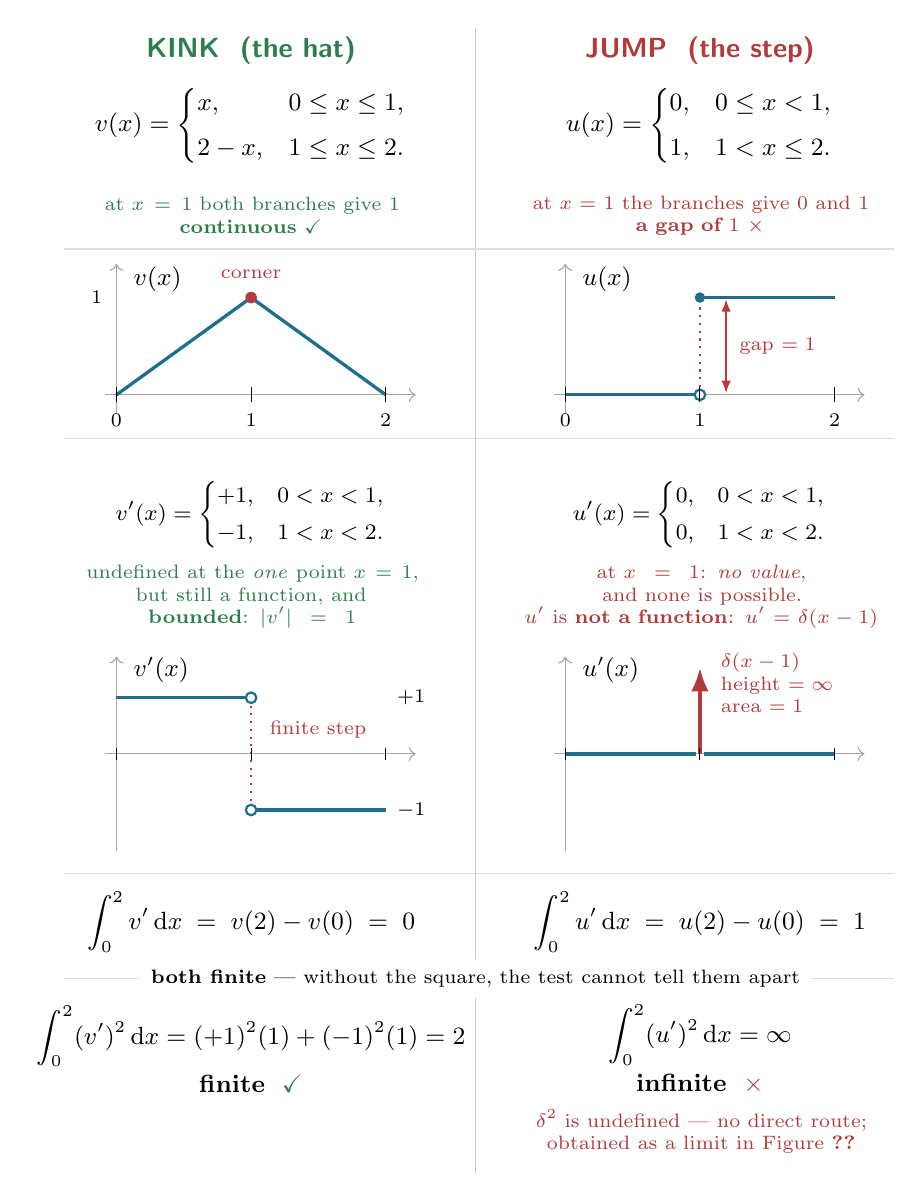
\begin{tikzpicture}[scale=0.95, every node/.style={font=\small}]

\node[font=\bfseries\sffamily, MEFrame]  at (2.0, 9.5) {KINK\ \ (the hat)};
\node[font=\bfseries\sffamily, PitFrame] at (8.0, 9.5) {JUMP\ \ (the step)};
\draw[gray!45] (5.0,-5.5) -- (5.0,9.8);
% faint row separators
\foreach \y in {6.85, 4.32, -1.5, -2.9}{\draw[gray!25] (-0.5,\y) -- (10.6,\y);}

% ---------- ROW 1 : the definitions ----------
\node[font=\small] at (2.0,8.5)
  {$\displaystyle v(x)=\begin{cases} x, & 0\le x\le 1,\\[3pt] 2-x, & 1\le x\le 2.\end{cases}$};
\node[font=\small] at (8.0,8.5)
  {$\displaystyle u(x)=\begin{cases} 0, & 0\le x< 1,\\[3pt] 1, & 1< x\le 2.\end{cases}$};

\node[font=\scriptsize,MEFrame,align=center,text width=4.4cm]  at (2.0,7.3)
  {at $x=1$ both branches give $1$\\ \textbf{continuous} \cmark};
\node[font=\scriptsize,PitFrame,align=center,text width=4.4cm] at (8.0,7.3)
  {at $x=1$ the branches give $0$ and $1$\\ \textbf{a gap of $1$} \xmark};

% ---------- ROW 3 : the derivative expressions ----------
\node[font=\footnotesize] at (2.0,3.3)
  {$\displaystyle v'(x)=\begin{cases} +1, & 0<x<1,\\[2pt] -1, & 1<x<2.\end{cases}$};
\node[font=\footnotesize] at (8.0,3.3)
  {$\displaystyle u'(x)=\begin{cases} 0, & 0<x<1,\\[2pt] 0, & 1<x<2.\end{cases}$};

\node[font=\scriptsize,MEFrame,align=center,text width=4.7cm]  at (2.0,2.2)
  {undefined at the \emph{one} point $x=1$,\\
   but still a function, and \textbf{bounded}: $\abs{v'}=1$};
\node[font=\scriptsize,PitFrame,align=center,text width=4.7cm] at (8.0,2.2)
  {at $x=1$: \emph{no value}, and none is possible.\\
   $u'$ is \textbf{not a function}: $u'=\delta(x-1)$};

% ================= LEFT : KINK =================
% --- shape ---
\begin{scope}[shift={(0.2,4.9)}]
  \draw[->,gray!70] (-0.15,0) -- (4.0,0);
  \draw[->,gray!70] (0,-0.25) -- (0,1.75);
  \draw[very thick,IntFrame] (0,0) -- (1.8,1.3) -- (3.6,0);
  \fill[PitFrame] (1.8,1.3) circle (2.2pt);
  \node[PitFrame,above,font=\scriptsize] at (1.8,1.42) {corner};
  \foreach \x/\l in {0/0, 1.8/1, 3.6/2}{\draw (\x,-0.1)--(\x,0.1); \node[below,font=\scriptsize] at (\x,-0.12) {$\l$};}
  \node[left,font=\scriptsize] at (-0.06,1.3) {$1$};
  \node[right,font=\small] at (0.1,1.55) {$v(x)$};
\end{scope}
% --- derivative ---
\begin{scope}[shift={(0.2,0.1)}]
  \draw[->,gray!70] (-0.15,0) -- (4.0,0);
  \draw[->,gray!70] (0,-1.3) -- (0,1.3);
  \draw[very thick,IntFrame] (0,0.75) -- (1.8,0.75);
  \draw[very thick,IntFrame] (1.8,-0.75) -- (3.6,-0.75);
  \draw[dotted,thick,PitFrame] (1.8,0.75) -- (1.8,-0.75);
  \draw[IntFrame,fill=white,thick] (1.8,0.75)  circle (2pt);
  \draw[IntFrame,fill=white,thick] (1.8,-0.75) circle (2pt);
  \node[right,font=\scriptsize] at (3.62,0.75)  {$+1$};
  \node[right,font=\scriptsize] at (3.62,-0.75) {$-1$};
  \node[PitFrame,right,font=\scriptsize] at (1.92,0.32) {finite step};
  \foreach \x/\l in {0/0, 1.8/1, 3.6/2}{\draw (\x,-0.08)--(\x,0.08);}
  \node[right,font=\small] at (0.1,1.12) {$v'(x)$};
\end{scope}
% --- row 5: the PLAIN integral (no square) ---
\node[align=center,font=\small] at (2.0,-2.15)
  {$\displaystyle\int_{0}^{2} v'\dx \;=\; v(2)-v(0) \;=\; 0$};
% --- row 6: the SQUARED integral ---
\node[align=center,font=\small] at (2.0,-3.85)
  {$\displaystyle\int_{0}^{2}(v')^{2}\dx = (+1)^{2}(1)+(-1)^{2}(1) = 2$\\[2pt]
   \textbf{finite} \ \cmark};

% ================= RIGHT : JUMP =================
% --- shape ---
\begin{scope}[shift={(6.2,4.9)}]
  \draw[->,gray!70] (-0.15,0) -- (4.0,0);
  \draw[->,gray!70] (0,-0.25) -- (0,1.75);
  \draw[very thick,IntFrame] (0,0) -- (1.8,0);
  \draw[very thick,IntFrame] (1.8,1.3) -- (3.6,1.3);
  \draw[dotted,thick,PitFrame] (1.8,0) -- (1.8,1.3);
  \draw[IntFrame,fill=white,thick] (1.8,0) circle (2pt);
  \fill[IntFrame] (1.8,1.3) circle (2pt);
  \draw[{Latex[length=1.6mm]}-{Latex[length=1.6mm]},PitFrame,thick] (2.15,0.02) -- (2.15,1.28);
  \node[PitFrame,right,font=\scriptsize] at (2.2,0.65) {gap $=1$};
  \foreach \x/\l in {0/0, 1.8/1, 3.6/2}{\draw (\x,-0.1)--(\x,0.1); \node[below,font=\scriptsize] at (\x,-0.12) {$\l$};}
  \node[right,font=\small] at (0.1,1.55) {$u(x)$};
\end{scope}
% --- derivative ---
\begin{scope}[shift={(6.2,0.1)}]
  \draw[->,gray!70] (-0.15,0) -- (4.0,0);
  \draw[->,gray!70] (0,-1.3) -- (0,1.3);
  \draw[very thick,IntFrame] (0,0) -- (1.75,0);
  \draw[very thick,IntFrame] (1.85,0) -- (3.6,0);
  \draw[very thick,-{Latex[length=3mm]},PitFrame] (1.8,0) -- (1.8,1.15);
  \node[PitFrame,right,font=\scriptsize,align=left] at (1.95,0.95) {$\delta(x-1)$\\ height $=\infty$\\ area $=1$};
  \foreach \x/\l in {0/0, 1.8/1, 3.6/2}{\draw (\x,-0.08)--(\x,0.08);}
  \node[right,font=\small] at (0.1,1.12) {$u'(x)$};
\end{scope}
% --- row 5: the PLAIN integral (no square) ---
\node[align=center,font=\small] at (8.0,-2.15)
  {$\displaystyle\int_{0}^{2} u'\dx \;=\; u(2)-u(0) \;=\; 1$};
% --- row 6: the SQUARED integral ---
\node[align=center,font=\small] at (8.0,-3.85)
  {$\displaystyle\int_{0}^{2}(u')^{2}\dx = \infty$\\[2pt] \textbf{infinite} \ \xmark};
\node[font=\scriptsize,PitFrame,align=center,text width=4.7cm] at (8.0,-4.95)
  {$\delta^{2}$ is undefined --- no direct route;\\
   obtained as a limit in Figure~\ref{fig:smooth}};

% --- the punchline, straddling both columns ---
\node[fill=white,inner sep=4pt,font=\scriptsize,align=center] at (5.0,-2.9)
  {\textbf{both finite} --- without the square, the test cannot tell them apart};

\end{tikzpicture}
\caption{Rows: definition, shape, $v'$ as a formula, $v'$ plotted, $\int v'$, $\int (v')^{2}$. Only the last row separates the two cases.}
\label{fig:master}
\end{figure}

\paragraph{The hat.} Differentiate each branch of \eqref{eq:two}:
\begin{equation}
  v'(x) = \begin{cases}
    +1, & x<1,\\
    \text{undefined}, & x=1 \quad(\text{left says }+1,\ \text{right says }-1),\\
    -1, & x>1 .
  \end{cases}
\end{equation}
It genuinely fails to exist --- at exactly one point. But
\begin{equation}
  \int_{0}^{2}(v')^{2}\dx = \int_{0}^{1}1\dx + \int_{1}^{2}1\dx = 2,
\end{equation}
because a single point has zero length and contributes nothing to an integral.
The value $v'(1)$ is never needed. Note also that $v'$ stays \textbf{bounded}:
it only ever takes the values $\pm1$.

\paragraph{The step.} Away from $x=1$ the function is flat, so $u'=0$. At
$x=1$ it changes by $1$ over a length of $0$:
\[
  \text{slope} = \frac{\text{rise}}{\text{run}} = \frac{1}{0} = \infty .
\]
That is not a number, so guessing is no good. Instead, approach it.

% ==================================================================
\section{Where the delta comes from: smooth the jump, then shrink}
\label{sec:smoothing}

Replace the instantaneous jump by a steep ramp of width $h$ centred at $x=1$:
\begin{equation}\label{eq:uh}
  u_{h}(x) = \begin{cases}
    0, & x \le 1-\tfrac{h}{2},\\[2pt]
    \dfrac{x-(1-h/2)}{h}, & 1-\tfrac{h}{2}\le x\le 1+\tfrac{h}{2},\\[6pt]
    1, & x \ge 1+\tfrac{h}{2}.
  \end{cases}
  \qquad\Longrightarrow\qquad
  u_{h}'(x) = \begin{cases}
    \dfrac{1}{h}, & \text{on the ramp,}\\[6pt]
    0, & \text{elsewhere.}
  \end{cases}
\end{equation}
So $u_{h}'$ is a rectangle of height $1/h$ and width $h$. Now shrink $h$.

\begin{figure}[htbp]
\centering
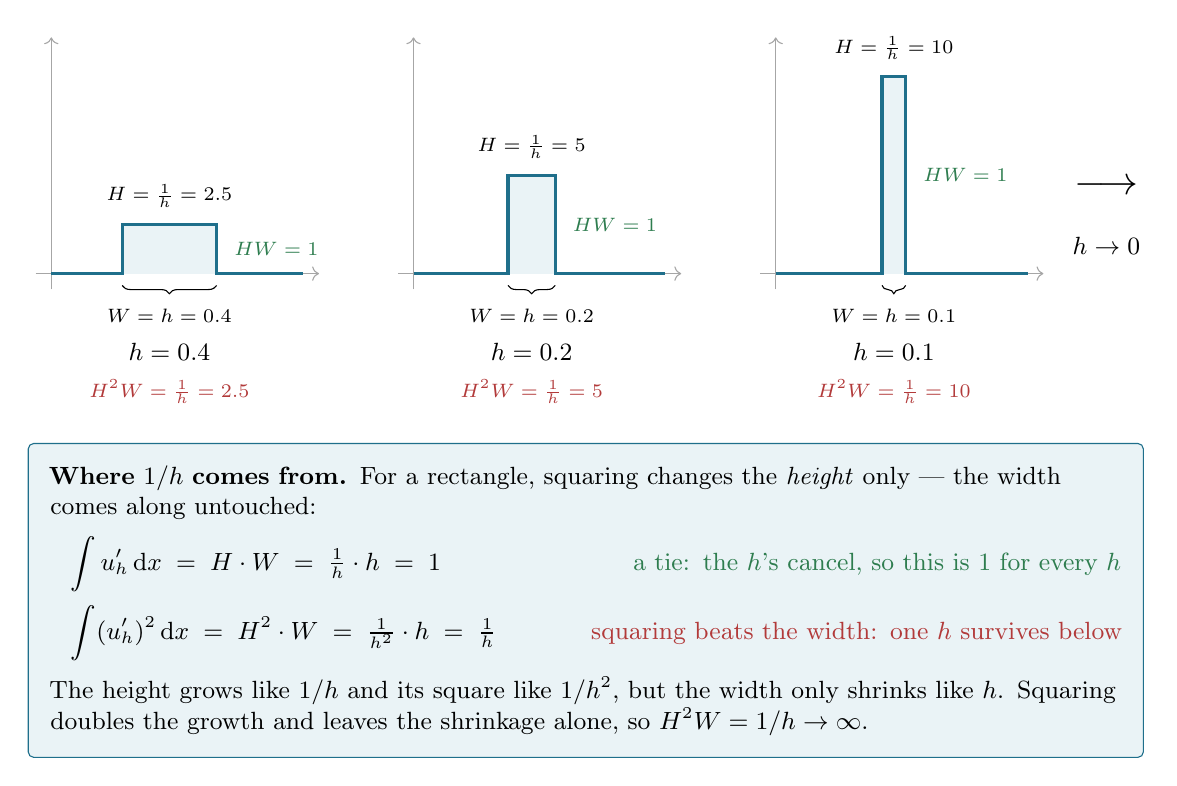
\begin{tikzpicture}[scale=1.0, every node/.style={font=\small}]
% three panels: h = 0.4, 0.2, 0.1 ; height 1/h scaled by 0.25 ; x-unit = 3cm
\foreach \i/\hh/\wdt/\hgt/\inv in {0/0.4/1.2/0.625/2.5, 1/0.2/0.6/1.25/5, 2/0.1/0.3/2.5/10}{
  \begin{scope}[shift={(\i*4.6,0)}]
    \draw[->,gray!70] (-0.2,0) -- (3.4,0);
    \draw[->,gray!70] (0,-0.2) -- (0,3.0);
    \fill[IntBack] (1.5-\wdt/2,0) rectangle (1.5+\wdt/2,\hgt);
    \draw[very thick,IntFrame] (0,0) -- (1.5-\wdt/2,0) -- (1.5-\wdt/2,\hgt)
        -- (1.5+\wdt/2,\hgt) -- (1.5+\wdt/2,0) -- (3.2,0);
    \node[font=\scriptsize,align=center] at (1.5,\hgt+0.36) {$H=\tfrac1h=\inv$};
    \draw[decorate,decoration={brace,amplitude=3pt,mirror},thin]
         (1.5-\wdt/2,-0.15) -- (1.5+\wdt/2,-0.15);
    \node[below,font=\scriptsize] at (1.5,-0.32) {$W=h=\hh$};
    \node[MEFrame,font=\scriptsize,right] at (1.5+\wdt/2+0.1,\hgt/2) {$HW=1$};
    \node[font=\small\bfseries] at (1.5,-1.0) {$h=\hh$};
    \node[font=\scriptsize,PitFrame] at (1.5,-1.5) {$H^{2}W=\tfrac{1}{h}=\inv$};
  \end{scope}
}
\node[font=\Large] at (13.4,1.1) {$\longrightarrow$};
\node[font=\small,align=center] at (13.4,0.35) {$h\to0$};

% ---- the H^2 W derivation, spelled out ----
\node[draw=IntFrame, fill=IntBack, rounded corners=2pt, inner sep=8pt,
      anchor=north west, align=left, text width=13.6cm, font=\small]
     at (-0.3,-2.15)
  {\textbf{Where $1/h$ comes from.} For a rectangle, squaring changes the
   \emph{height} only --- the width comes along untouched:
   \\[5pt]
   \hspace*{0.8em}$\displaystyle\int u_{h}'\dx \;=\; H\cdot W
     \;=\;\tfrac{1}{h}\cdot h \;=\; 1$
   \hfill\textcolor{MEFrame}{a tie: the $h$'s cancel, so this is $1$ for every $h$}
   \\[4pt]
   \hspace*{0.8em}$\displaystyle\int (u_{h}')^{2}\dx \;=\; H^{2}\cdot W
     \;=\;\tfrac{1}{h^{2}}\cdot h \;=\; \tfrac{1}{h}$
   \hfill\textcolor{PitFrame}{squaring beats the width: one $h$ survives below}
   \\[5pt]
   The height grows like $1/h$ and its square like $1/h^{2}$, but the width only
   shrinks like $h$. Squaring doubles the growth and leaves the shrinkage alone,
   so $H^{2}W=1/h\to\infty$.};
\end{tikzpicture}
\caption{Shrinking $h$. Height $H=1/h$, width $W=h$, so $HW=1$ always --- but $H^{2}W=1/h\to\infty$.}
\label{fig:smooth}
\end{figure}

\begin{center}
\renewcommand{\arraystretch}{1.25}
\begin{tabular}{@{}rrrrr@{}}
\toprule
$h$ & height $H=\tfrac1h$ & width $W=h$
    & $\displaystyle\int u_{h}'\dx = HW$
    & $\displaystyle\int (u_{h}')^{2}\dx = H^{2}W$\\
\midrule
$0.1$    & $10$   & $0.1$   & $1$ & $10$\\
$0.01$   & $100$  & $0.01$  & $1$ & $100$\\
$0.001$  & $1000$ & $0.001$ & $1$ & $1000$\\
\midrule
$\to 0$  & $\to\infty$ & $\to 0$ & $\mathbf{1}$ & $\boldsymbol{\to\infty}$\\
\bottomrule
\end{tabular}
\end{center}

\medskip
Three things happen at once:
\begin{enumerate}[label=(\arabic*),leftmargin=2em,itemsep=1pt]
  \item the height $\to\infty$;
  \item the width $\to 0$;
  \item the \textbf{area stays exactly $1$} --- always, since $(1/h)\cdot h=1$.
\end{enumerate}

\begin{intuition}[what a ``delta spike'' actually is]
The limit is the \textbf{Dirac delta} $\delta(x-1)$: infinite height, zero
width, area $1$.

It is \emph{not a function} --- ordinary integration cannot see a single point,
so no function can be infinite there and still enclose area $1$. It is defined
only by what it does inside an integral:
\[
  \int \delta(x-x_{0})\dx = 1
  \qquad\text{(unit area)},
  \qquad
  \int f(x)\,\delta(x-x_{0})\dx = f(x_{0})
  \qquad\text{(samples $f$ at $x_{0}$)} .
\]
Hence it is drawn as an \textbf{arrow}: the arrow's height on the page is its
\emph{area}, not its height. Height $3$ means $3\delta$.

\textbf{The derivative of a step is a delta.}
\end{intuition}

\begin{pitfall}[never write ``$u'(1)=\infty$'' --- it gives the wrong integral]
It is tempting to record the spike as a pointwise value:
\[
  u'(x)=\begin{cases} 0, & x\ne1,\\ \infty, & x=1.\end{cases}
  \qquad\text{\xmark\ \textbf{This is not merely sloppy --- it is false.}}
\]
Decisive test --- FTC pins the answer at $\int_{0}^{2}u'\dx = u(2)-u(0) = 1$.
But that formula is a genuine function, zero except at one point, and a single
point has zero width, so it contributes nothing \emph{whatever} value sits there
($\infty$ included):
\[
  \int_{0}^{2} u'\dx = 0 \;\ne\; 1 .
\]
Writing $\infty$ destroys the one property that makes $\delta$ worth having.
\begin{center}\small
\renewcommand{\arraystretch}{1.25}
\begin{tabular}{@{}lll@{}}
\toprule
\textbf{Phrasing} & \textbf{Verdict} & \textbf{Why}\\
\midrule
$u'(1)=\infty$ & \xmark\ wrong & yields $\int u'=0$ instead of $1$\\
$u'(1)$ undefined, ``$1/0$'' & partly right & honest, and the ``$1$'' is really
   the area --- but it\\
 & & is not a value, and it loses the \emph{location}\\
$u'(1)$ has \emph{no value} & \cmark\ correct & accurate, though it sounds
   emptier than the truth\\
\bottomrule
\end{tabular}
\end{center}

\noindent
All three share the same false premise: $u'$ is not a function, so it has no
entries at points to fill in. The honest statement is two lines:
\[
  u'(x)=0 \ \text{ for } x\ne1,
  \qquad\text{and, as a distribution,}\qquad
  u'=\delta(x-1),
\]
the second carrying what the first cannot --- \emph{where} ($1$) and
\emph{how much} (area $1$). Keep ``$1/0$'' as scaffolding: a jump of size $3$
gives $3/0$ and yields $3\delta(x-1)$, so the numerator is the coefficient.
\end{pitfall}

% ==================================================================
\section{Why the kink stays tame: the same experiment on the hat}

Do the identical smoothing to the hat's corner --- let $v_{h}'$ ramp linearly
from $+1$ down to $-1$ across a window of width $h$.

\begin{figure}[htbp]
\centering
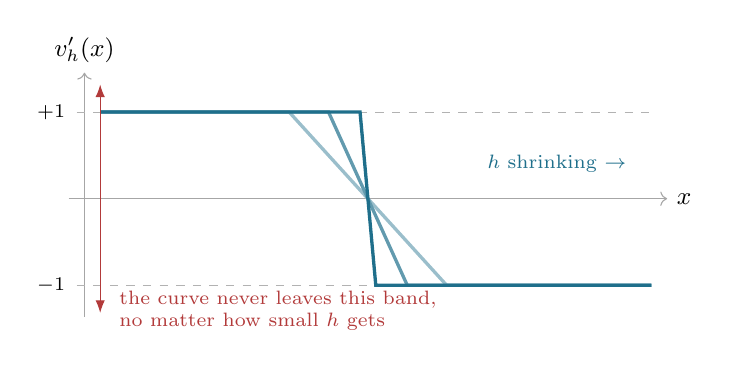
\begin{tikzpicture}[scale=1.0, every node/.style={font=\small}]
  \draw[->,gray!70] (-0.2,0) -- (7.4,0) node[right,font=\small,black] {$x$};
  \draw[->,gray!70] (0,-1.5) -- (0,1.6) node[above,font=\small,black] {$v_{h}'(x)$};
  \draw[dashed,gray!60] (-0.1,1.1) -- (7.2,1.1);
  \draw[dashed,gray!60] (-0.1,-1.1) -- (7.2,-1.1);
  \node[left,font=\scriptsize] at (-0.12,1.1)  {$+1$};
  \node[left,font=\scriptsize] at (-0.12,-1.1) {$-1$};
  % three transitions of shrinking width, all bounded by +-1
  \draw[very thick,IntFrame!45] (0.2,1.1) -- (2.6,1.1) -- (4.6,-1.1) -- (7.2,-1.1);
  \draw[very thick,IntFrame!70] (0.2,1.1) -- (3.1,1.1) -- (4.1,-1.1) -- (7.2,-1.1);
  \draw[very thick,IntFrame]    (0.2,1.1) -- (3.5,1.1) -- (3.7,-1.1) -- (7.2,-1.1);
  \node[font=\scriptsize,IntFrame] at (6.0,0.45) {$h$ shrinking $\rightarrow$};
  \draw[{Latex[length=1.6mm]}-{Latex[length=1.6mm]},PitFrame] (0.2,1.45) -- (0.2,-1.45);
  \node[PitFrame,right,font=\scriptsize,align=left] at (0.32,-1.42)
       {the curve never leaves this band,\\ no matter how small $h$ gets};
\end{tikzpicture}
\caption{The same smoothing on the kink: $v_{h}'$ never leaves $[-1,+1]$, so nothing can blow up.}
\label{fig:kinksmooth}
\end{figure}

\begin{center}
\renewcommand{\arraystretch}{1.25}
\begin{tabular}{@{}rrr@{}}
\toprule
$h$ & $\max\abs{v_{h}'}$ & $\displaystyle\int_{0}^{2}(v_{h}')^{2}\dx = 2-\tfrac{2h}{3}$\\
\midrule
$0.1$   & $1$ & $1.933$\\
$0.01$  & $1$ & $1.993$\\
$0.001$ & $1$ & $1.9993$\\
\midrule
$\to0$  & $\mathbf{1}$ & $\boldsymbol{\to 2}$ \quad(finite)\\
\bottomrule
\end{tabular}
\end{center}

\medskip\noindent
\textbf{The height never grows.} That single fact is the whole difference.
Squaring a bounded function leaves a bounded function, and a bounded function on
a bounded interval has a finite integral. Squaring a spike of height $1/h$ gives
$1/h^{2}$, and multiplying by the width $h$ still leaves $1/h\to\infty$.

% ==================================================================
\section{Auditing the four integrals: when may you split at the break?}
\label{sec:audit}

Every entry in the last two rows of Figure~\ref{fig:master} was reached by the
same instinct --- \emph{split the domain at $x=1$, integrate each piece, add}:
\begin{equation}\label{eq:naive}
  \int_{0}^{2} (\,\cdot\,)\dx
  \;\overset{?}{=}\;
  \int_{0}^{1} (\,\cdot\,)\dx \;+\; \int_{1}^{2} (\,\cdot\,)\dx
  \qquad\text{\emph{the naive piecewise method.}}
\end{equation}
Run it on all four cells, checking each against something known independently.
Two pass, two fail --- along exactly the kink/jump line.

% ------------------------------------------------------------------
\subsection*{(1) $\int_{0}^{2} v'\dx$ --- \textcolor{MEFrame}{\textbf{PASS}}}

On $(0,1)$, $v'$ is the constant $+1$ (antiderivative $x$); on $(1,2)$ it is the
constant $-1$ (antiderivative $-x$):
\[
  \int_{0}^{1}(+1)\dx + \int_{1}^{2}(-1)\dx
  = \bigl[x\bigr]_{0}^{1} + \bigl[-x\bigr]_{1}^{2}
  = (1-0) + \bigl((-2)-(-1)\bigr)
  = 1 - 1 = 0 .
\]
\textbf{Independent check.} The fundamental theorem gives
$v(2)-v(0) = 0-0 = 0$. \ \textbf{Agrees.}

\textbf{Why.} The split discards $x=1$; there $v'$ is \emph{bounded}, and zero
width $\times$ bounded height contributes nothing.

% ------------------------------------------------------------------
\subsection*{(2) $\int_{0}^{2} (v')^{2}\dx$ --- \textcolor{MEFrame}{\textbf{PASS}}}

Square first: $(+1)^{2}=1$ and $(-1)^{2}=1$, so \emph{both} pieces have
antiderivative $x$:
\[
  \int_{0}^{1}(+1)^{2}\dx + \int_{1}^{2}(-1)^{2}\dx
  = \bigl[x\bigr]_{0}^{1} + \bigl[x\bigr]_{1}^{2}
  = (1-0) + (2-1)
  = 1 + 1 = 2 .
\]
\textbf{Independent check.} $(v')^{2}=1$ at every point except $x=1$, so the
integrand is just the constant $1$ and $\int_{0}^{2}1\dx = 2$. \ \textbf{Agrees.}

\textbf{Why.} Same reason --- the square of a bounded function is still
bounded.

\begin{remark}
Comparing (1) and (2): identical structure, and the only difference is the
antiderivative of the second piece --- $-x$ becomes $+x$, because $(-1)^{2}=+1$.
That single sign change turns cancellation ($1-1=0$) into accumulation
($1+1=2$).
\end{remark}

% ------------------------------------------------------------------
\subsection*{(3) $\int_{0}^{2} u'\dx$ --- \textcolor{PitFrame}{\textbf{FAIL}}}

On both open pieces $u'=0$:
\[
  \int_{0}^{1} 0\dx + \int_{1}^{2} 0\dx = 0 + 0 = 0 .
\]
\textbf{Independent check.} The fundamental theorem gives
$u(2)-u(0) = 1-0 = 1$.
\[
  0 \;\ne\; 1 \qquad \text{\xmark\ \textbf{the method has lost the entire answer.}}
\]

\textbf{Why.} The split assumes nothing happens at $x=1$ --- true for $v'$,
false here. The pieces are empty; the whole answer sits at $x=1$ as the unit
area of $\delta(x-1)$.

% ------------------------------------------------------------------
\subsection*{(4) $\int_{0}^{2} (u')^{2}\dx$ --- \textcolor{PitFrame}{\textbf{FAIL}}}

Squaring zero changes nothing, so the naive method again returns
\[
  \int_{0}^{1} 0\dx + \int_{1}^{2} 0\dx = 0 .
\]
\textbf{Independent check.} The smoothing of \S\ref{sec:smoothing} gives
$\int_{0}^{2}(u_{h}')^{2}\dx = 1/h \to \infty$.
\[
  0 \;\ne\; \infty \qquad \text{\xmark}
\]
\textbf{Why.} Same illegal split; what sits at $x=1$ is now unbounded, so
discarding it turns $\infty$ into $0$. And $(u')^{2}$ is not the derivative of
anything, so there is no FTC fallback --- smoothing is the \emph{only} route
here.

% ------------------------------------------------------------------
\subsection*{The scorecard}

\begin{center}
\renewcommand{\arraystretch}{1.3}
\begin{tabular}{@{}llll l@{}}
\toprule
\textbf{Integral} & \textbf{Naive gives} & \textbf{True value} &
\textbf{Verdict} & \textbf{Checked against}\\
\midrule
$\int_{0}^{2} v'\dx$      & $0$ & $0$      & \textcolor{MEFrame}{\textbf{pass}} \cmark & FTC\\
$\int_{0}^{2} (v')^{2}\dx$& $2$ & $2$      & \textcolor{MEFrame}{\textbf{pass}} \cmark & direct ($(v')^{2}\equiv1$)\\
$\int_{0}^{2} u'\dx$      & $0$ & $1$      & \textcolor{PitFrame}{\textbf{fail}} \xmark & FTC\\
$\int_{0}^{2} (u')^{2}\dx$& $0$ & $\infty$ & \textcolor{PitFrame}{\textbf{fail}} \xmark & the limit, Figure~\ref{fig:smooth}\\
\bottomrule
\end{tabular}
\end{center}

\begin{intuition}[the pass/fail line \emph{is} the kink/jump line]
Splitting at $x=1$ and integrating only the two open pieces silently discards
the split point. So \eqref{eq:naive} is legitimate exactly when that point
contributes nothing:
\begin{center}\small
\renewcommand{\arraystretch}{1.25}
\begin{tabular}{@{}ll@{}}
\toprule
\textbf{The hat} ($v'$ \emph{bounded}) & \textbf{The step} ($u'$ a \emph{delta})\\
\midrule
zero width $\times$ height at most $1$ & the pieces are empty --- \emph{all}\\
$=$ zero contribution & the content sits at $x=1$\\
discarding it is harmless & discarding it discards everything\\
\textcolor{MEFrame}{\textbf{splitting is legal}} & \textcolor{PitFrame}{\textbf{splitting is illegal}}\\
\bottomrule
\end{tabular}
\end{center}

\noindent
\textbf{The naive method passes on a kink and fails on a jump} --- for both
integrals. Splitting at a break asserts that nothing lives there: true for a
kink, false for a jump, and the method then returns a wrong answer silently.
\end{intuition}

\section{The verdict}

\begin{dictbox}[kink vs.\ jump, everything at once]
\renewcommand{\arraystretch}{1.3}
\begin{tabularx}{\linewidth}{@{}l>{\raggedright\arraybackslash}X>{\raggedright\arraybackslash}X@{}}
\toprule
 & \textbf{KINK} (hat) & \textbf{JUMP} (step)\\
\midrule
what is broken            & the \emph{slope} $v'$        & the \emph{shape} $v$ itself\\
$v$ is                    & continuous                   & discontinuous\\
$v'$ near the break       & \emph{steps} $+1\to-1$       & \emph{spikes} to $1/h$\\
height of $v'$            & bounded (always $1$)         & unbounded ($\to\infty$)\\
$v'$ is                   & a function                   & a delta --- not a function\\
$\int v'\dx$              & $0$                          & $1$ \ (finite!)\\
$\int (v')^{2}\dx$        & $2$ \quad finite \cmark      & $\infty$ \quad \xmark\\
in $V$?                   & \textbf{yes}                 & \textbf{no}\\
mechanically              & a \textbf{material interface} --- steel glued to aluminium: displacement continuous, strain jumps because $E$ jumps & a \textbf{broken bar} --- a gap has opened; the structure has come apart\\
\bottomrule
\end{tabularx}
\end{dictbox}

\begin{pitfall}[the jump is finite --- the \emph{energy} is what is infinite]
Look at the two integral rows above. For the step,
\[
  \int u'\dx = 1 \quad\text{(finite)},
  \qquad\qquad
  \int (u')^{2}\dx = \infty .
\]
The displacement jump itself is a perfectly ordinary number: the bar opened by
$1$. What diverges is the \emph{square}. A delta has finite area but infinite
squared area.

This is precisely why the admissibility test is written with a square. Had the
condition been $\int v'\dx<\infty$, the broken bar would have passed --- and
the theory would admit configurations in which the structure has come apart.
The square is what makes $V$ physical, because the square is the energy.
\end{pitfall}

% ==================================================================
\section{Climbing the ladder: $v$, $v'$, $v''$}

The rule ``differentiating a step produces a delta'' can be applied twice.
Take the finite element hat --- the same function, now extended by zero outside
$[0,2]$, as it actually appears in a mesh.

\begin{figure}[htbp]
\centering
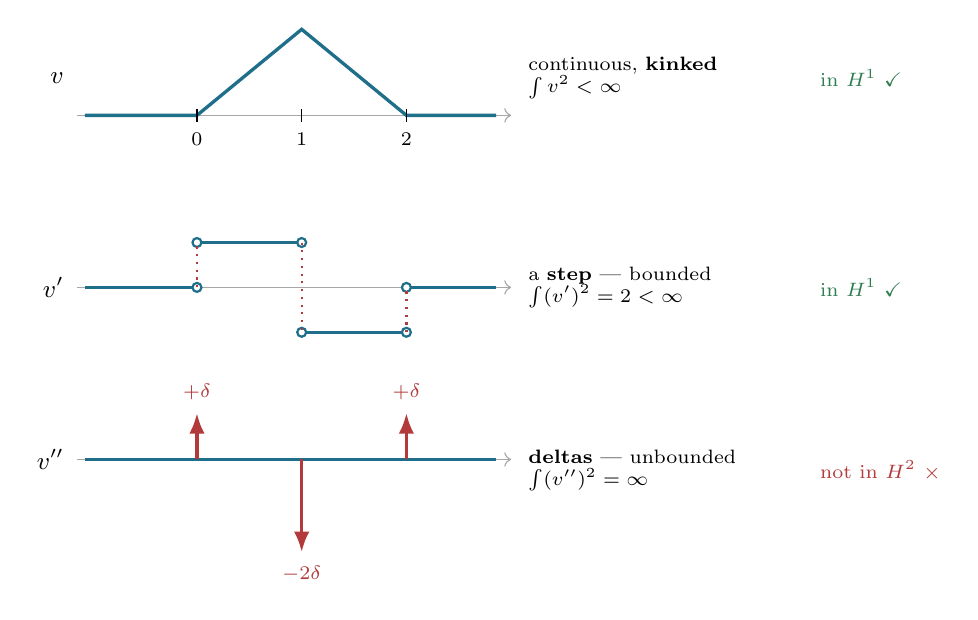
\begin{tikzpicture}[scale=0.95, every node/.style={font=\small}]

% ---- v ----
\begin{scope}[shift={(0,4.6)}]
  \draw[->,gray!70] (-0.4,0) -- (5.4,0);
  \draw[very thick,IntFrame] (-0.3,0) -- (1.2,0) -- (2.6,1.15) -- (4.0,0) -- (5.2,0);
  \foreach \x/\l in {1.2/0, 2.6/1, 4.0/2}{\draw (\x,-0.09)--(\x,0.09); \node[below,font=\scriptsize] at (\x,-0.11) {$\l$};}
  \node[left,font=\small] at (-0.45,0.5) {$v$};
  \node[right,align=left,font=\scriptsize] at (5.5,0.5)
    {continuous, \textbf{kinked}\\ $\int v^{2}<\infty$};
  \node[right,MEFrame,font=\scriptsize] at (9.4,0.5) {in $H^{1}$ \cmark};
\end{scope}

% ---- v' ----
\begin{scope}[shift={(0,2.3)}]
  \draw[->,gray!70] (-0.4,0) -- (5.4,0);
  \draw[very thick,IntFrame] (-0.3,0) -- (1.2,0);
  \draw[very thick,IntFrame] (1.2,0.6) -- (2.6,0.6);
  \draw[very thick,IntFrame] (2.6,-0.6) -- (4.0,-0.6);
  \draw[very thick,IntFrame] (4.0,0) -- (5.2,0);
  \foreach \p in {(1.2,0),(1.2,0.6),(2.6,0.6),(2.6,-0.6),(4.0,-0.6),(4.0,0)}
    {\draw[IntFrame,fill=white,thick] \p circle (1.7pt);}
  \draw[dotted,PitFrame,thick] (1.2,0)--(1.2,0.6);
  \draw[dotted,PitFrame,thick] (2.6,0.6)--(2.6,-0.6);
  \draw[dotted,PitFrame,thick] (4.0,-0.6)--(4.0,0);
  \node[left,font=\small] at (-0.45,0) {$v'$};
  \node[right,align=left,font=\scriptsize] at (5.5,0)
    {a \textbf{step} --- bounded\\ $\int (v')^{2}=2<\infty$};
  \node[right,MEFrame,font=\scriptsize] at (9.4,0) {in $H^{1}$ \cmark};
\end{scope}

% ---- v'' ----
\begin{scope}[shift={(0,0)}]
  \draw[->,gray!70] (-0.4,0) -- (5.4,0);
  \draw[very thick,IntFrame] (-0.3,0) -- (5.2,0);
  \draw[very thick,-{Latex[length=2.6mm]},PitFrame] (1.2,0) -- (1.2,0.62);
  \draw[very thick,-{Latex[length=2.6mm]},PitFrame] (2.6,0) -- (2.6,-1.24);
  \draw[very thick,-{Latex[length=2.6mm]},PitFrame] (4.0,0) -- (4.0,0.62);
  \node[PitFrame,above,font=\scriptsize] at (1.2,0.66) {$+\delta$};
  \node[PitFrame,below,font=\scriptsize] at (2.6,-1.3) {$-2\delta$};
  \node[PitFrame,above,font=\scriptsize] at (4.0,0.66) {$+\delta$};
  \node[left,font=\small] at (-0.45,0) {$v''$};
  \node[right,align=left,font=\scriptsize] at (5.5,-0.15)
    {\textbf{deltas} --- unbounded\\ $\int (v'')^{2}=\infty$};
  \node[right,PitFrame,font=\scriptsize] at (9.4,-0.15) {not in $H^{2}$ \xmark};
\end{scope}

\end{tikzpicture}
\caption{Differentiating the hat twice: kinked $\to$ bounded step $\to$ deltas. In $H^{1}$, not in $H^{2}$.}
\label{fig:ladder}
\end{figure}

\begin{equation}
  v'' = \delta(x) - 2\,\delta(x-1) + \delta(x-2).
\end{equation}
The coefficients are just the jumps in $v'$: it steps $0\to+1$ at $x=0$
(hence $+\delta$), then $+1\to-1$ at $x=1$ (a drop of $2$, hence $-2\delta$),
then $-1\to0$ at $x=2$ (hence $+\delta$).

\begin{intuition}[the hat is in $H^{1}$ but not in $H^{2}$]
This settles the bar/beam question that otherwise looks like a separate rule.
\begin{itemize}[leftmargin=1.4em,itemsep=2pt]
  \item $H^{1}$ requires $\int(v')^{2}<\infty$. The hat gives $2$. \textbf{Pass}
        --- so the hat is a legal \emph{bar} displacement, and a legal FE shape
        function for a bar, a truss, a solid, or a heat conduction problem.
  \item $H^{2}$ requires $\int(v'')^{2}<\infty$. The hat gives $\infty$.
        \textbf{Fail} --- so the hat is \emph{not} a legal \emph{beam}
        deflection.
\end{itemize}
Physically: a hat-shaped beam has a corner, so its curvature $v''$ is a delta
and $\tfrac12\int EI(v'')^{2}=\infty$. A hat-shaped beam is a \textbf{hinge}.
\end{intuition}

% ==================================================================
\section{Reading the $C^{k}$ labels off a polynomial}

A single polynomial is $C^{\infty}$. The classes appear only when you
\emph{glue} one to zero:
\begin{equation}\label{eq:trunc}
  f(x)=\begin{cases} x^{n}, & x\ge 0,\\ 0, & x<0,\end{cases}
  \qquad\text{on } [-1,1].
\end{equation}

\begin{center}\small
\renewcommand{\arraystretch}{1.25}
\begin{tabular}{@{}c cccc c@{}}
\toprule
$f\ (x\ge0)$ & $f$ & $f'$ & $f''$ & $f'''$ & \textbf{class of $f$}\\
\midrule
$1$       & \textcolor{PitFrame}{\textbf{JUMP}} & --- & --- & --- & $C^{-1}$\\
$x$       & kink & \textcolor{PitFrame}{\textbf{JUMP}} & --- & --- & $C^{0}$\\
$x^{2}$   & smooth & kink & \textcolor{PitFrame}{\textbf{JUMP}} & --- & $C^{1}$\\
$x^{3}$   & smooth & smooth & kink & \textcolor{PitFrame}{\textbf{JUMP}} & $C^{2}$\\
\midrule
$x^{k+1}$ & \multicolumn{4}{c}{\emph{the break marches one column right per power}} & $C^{k}$\\
\bottomrule
\end{tabular}
\end{center}

\noindent
\textbf{Rule.} If $f^{(m)}$ is the first derivative to jump, then
$f\in C^{m-1}$. So $x^{n}$ glued to zero is exactly $C^{n-1}$: each extra power
flattens the join by one more order.

\begin{figure}[htbp]
\centering
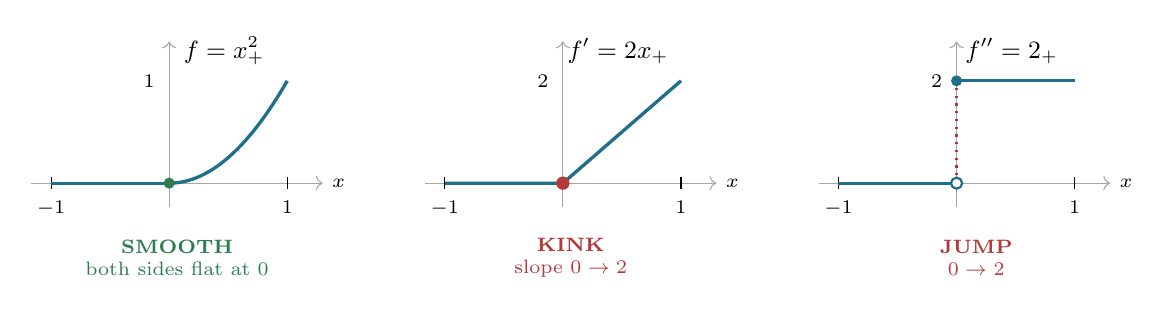
\begin{tikzpicture}[scale=1.0, every node/.style={font=\small}]
\foreach \i/\ttl in {0/{$f=x^{2}_{+}$}, 1/{$f'=2x_{+}$}, 2/{$f''=2_{+}$}}{
  \begin{scope}[shift={(\i*5.0,0)}]
    \draw[->,gray!70] (-1.75,0) -- (1.95,0) node[right,font=\scriptsize,black] {$x$};
    \draw[->,gray!70] (0,-0.3) -- (0,1.8);
    \foreach \x/\l in {-1.5/{-1}, 1.5/{1}}{
      \draw (\x,-0.08) -- (\x,0.08);
      \node[below,font=\scriptsize] at (\x,-0.1) {$\l$};}
    \node[font=\small] at (0.7,1.68) {\ttl};
  \end{scope}
}
% panel 1 : f = x^2  -- smooth
\begin{scope}
  \draw[very thick,IntFrame] (-1.5,0) -- (0,0);
  \draw[very thick,IntFrame,domain=0:1.5,samples=60]
        plot (\x,{1.3*(\x/1.5)*(\x/1.5)});
  \fill[MEFrame] (0,0) circle (2pt);
  \node[left,font=\scriptsize] at (-0.06,1.3) {$1$};
  \node[MEFrame,font=\scriptsize,align=center] at (0.1,-0.95)
       {\textbf{SMOOTH}\\ both sides flat at $0$};
\end{scope}
% panel 2 : f' = 2x -- kink
\begin{scope}[shift={(5.0,0)}]
  \draw[very thick,IntFrame] (-1.5,0) -- (0,0) -- (1.5,1.3);
  \fill[PitFrame] (0,0) circle (2.4pt);
  \node[left,font=\scriptsize] at (-0.06,1.3) {$2$};
  \node[PitFrame,font=\scriptsize,align=center] at (0.1,-0.95)
       {\textbf{KINK}\\ slope $0\to2$};
\end{scope}
% panel 3 : f'' = 2 -- jump
\begin{scope}[shift={(10.0,0)}]
  \draw[very thick,IntFrame] (-1.5,0) -- (0,0);
  \draw[very thick,IntFrame] (0,1.3) -- (1.5,1.3);
  \draw[dotted,thick,PitFrame] (0,0) -- (0,1.3);
  \draw[IntFrame,fill=white,thick] (0,0) circle (2pt);
  \fill[IntFrame] (0,1.3) circle (2pt);
  \node[left,font=\scriptsize] at (-0.06,1.3) {$2$};
  \node[PitFrame,font=\scriptsize,align=center] at (0.25,-0.95)
       {\textbf{JUMP}\\ $0\to2$};
\end{scope}
\end{tikzpicture}
\caption{$f=x^{2}_{+}$ is exactly $C^{1}$: invisible in $f$, a kink in $f'$, a
jump only in $f''$.}
\label{fig:ck}
\end{figure}

\begin{pitfall}[``kink'' and ``jump'' are relative --- say \emph{in what}]
A kink in $f$ \emph{is} a jump in $f'$ --- one event, named one level apart.

Figure~\ref{fig:ck} is the case that catches people: $f=x^{2}_{+}$ looks
perfectly smooth, because both sides are flat at $0$. The defect cannot be seen
in $f$ at all; you must differentiate twice to reach it.

Which is why beams are subtler than bars --- a beam deflection can look smooth
while its \emph{curvature} $w''$ is the broken quantity.
\end{pitfall}

\section{What this decides in finite element analysis}

Where each piece lands in practice.

% ------------------------------------------------------------------
\subsection{Why the basis functions are hats in the first place}

The chain runs backwards from what the method needs:
\begin{center}\small
\renewcommand{\arraystretch}{1.2}
\begin{tabular}{@{}rl@{}}
\toprule
want & a sparse, banded stiffness matrix\\
$\Rightarrow$ & basis functions with \emph{small support} (each touches few neighbours)\\
$\Rightarrow$ & the simplest such shape: the piecewise-linear \textbf{hat}\\
$\Rightarrow$ & hats have \emph{kinks}, so they are not $C^{1}$\\
$\Rightarrow$ & the admissible space must \textbf{tolerate kinks}\\
$\Rightarrow$ & use an \emph{energy} (integral) test, not a \emph{smoothness} (pointwise) test\\
$\Rightarrow$ & $V=H^{1}_{0}$\\
\bottomrule
\end{tabular}
\end{center}

\noindent
$H^{1}$ was reverse-engineered to be exactly big enough to hold hats and small
enough to exclude broken bars. Insist on classical differentiability and
piecewise-linear FEM becomes illegal: you would need globally smooth basis
functions, whose global support destroys sparsity.

\begin{figure}[htbp]
\centering
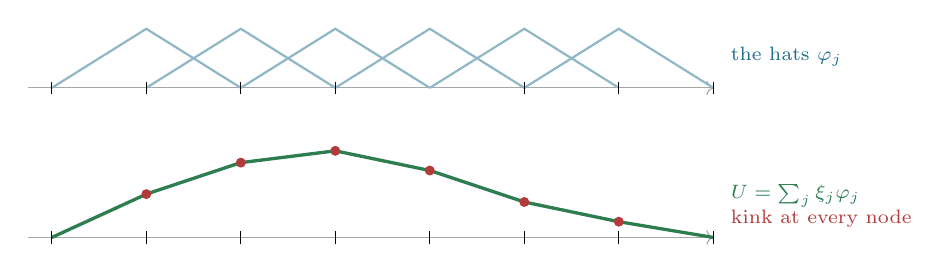
\begin{tikzpicture}[scale=1.0, every node/.style={font=\small}]
  % overlapping hats
  \begin{scope}[shift={(0,1.9)}]
    \draw[->,gray!70] (-0.3,0) -- (8.4,0);
    \foreach \c in {1.2,2.4,3.6,4.8,6.0,7.2}{
      \draw[IntFrame!50,thick] (\c-1.2,0) -- (\c,0.75) -- (\c+1.2,0);}
    \foreach \x/\l in {0/x_{0}, 1.2/x_{1}, 2.4/x_{2}, 3.6/x_{3}, 6.0/x_{M}, 7.2/{}, 8.4/{}}
      {\draw (\x,-0.08)--(\x,0.08);}
    \node[right,font=\scriptsize,IntFrame] at (8.5,0.4) {the hats $\phih_{j}$};
  \end{scope}
  % resulting FE solution
  \begin{scope}[shift={(0,0)}]
    \draw[->,gray!70] (-0.3,0) -- (8.4,0);
    \draw[very thick,MEFrame] (0,0) -- (1.2,0.55) -- (2.4,0.95) -- (3.6,1.1)
      -- (4.8,0.85) -- (6.0,0.45) -- (7.2,0.2) -- (8.4,0);
    \foreach \x/\y in {1.2/0.55, 2.4/0.95, 3.6/1.1, 4.8/0.85, 6.0/0.45, 7.2/0.2}
      {\fill[PitFrame] (\x,\y) circle (1.8pt);}
    \foreach \x in {0,1.2,2.4,3.6,4.8,6.0,7.2,8.4}{\draw (\x,-0.08)--(\x,0.08);}
    \node[right,font=\scriptsize,MEFrame,align=left] at (8.5,0.4)
      {$U=\sum_j \xi_j\phih_j$\\ \textcolor{PitFrame}{kink at every node}};
  \end{scope}
\end{tikzpicture}
\caption{The FE solution is a sum of hats --- a kink at every node, all legal. It must never \emph{jump}.}
\label{fig:fesum}
\end{figure}

% ------------------------------------------------------------------
\subsection{The compatibility rule: what element assembly is really enforcing}

\begin{figure}[htbp]
\centering
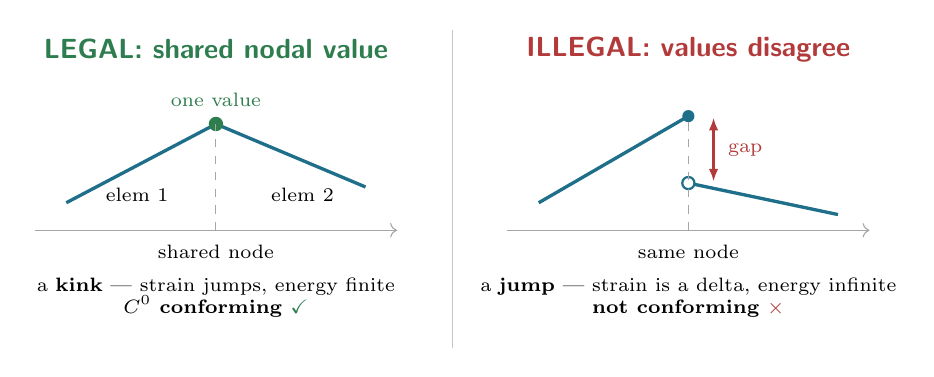
\begin{tikzpicture}[scale=1.0, every node/.style={font=\small}]

\node[font=\bfseries\sffamily,MEFrame]  at (2.1,2.3) {LEGAL: shared nodal value};
\node[font=\bfseries\sffamily,PitFrame] at (8.1,2.3) {ILLEGAL: values disagree};
\draw[gray!45] (5.1,-1.5) -- (5.1,2.55);

% --- legal ---
\begin{scope}[shift={(0,0)}]
  \draw[->,gray!70] (-0.2,0) -- (4.4,0);
  \draw[very thick,IntFrame] (0.2,0.35) -- (2.1,1.35);
  \draw[very thick,IntFrame] (2.1,1.35) -- (4.0,0.55);
  \fill[MEFrame] (2.1,1.35) circle (2.6pt);
  \draw[dashed,gray!70] (2.1,0) -- (2.1,1.35);
  \node[below,font=\scriptsize] at (2.1,-0.06) {shared node};
  \node[above,font=\scriptsize,MEFrame] at (2.1,1.45) {one value};
  \node[font=\scriptsize] at (1.1,0.45) {elem 1};
  \node[font=\scriptsize] at (3.2,0.45) {elem 2};
  \node[align=center,font=\scriptsize] at (2.1,-0.85)
    {a \textbf{kink} --- strain jumps, energy finite\\ \textbf{$C^{0}$ conforming} \cmark};
\end{scope}

% --- illegal ---
\begin{scope}[shift={(6.0,0)}]
  \draw[->,gray!70] (-0.2,0) -- (4.4,0);
  \draw[very thick,IntFrame] (0.2,0.35) -- (2.1,1.45);
  \draw[very thick,IntFrame] (2.1,0.6) -- (4.0,0.2);
  \draw[IntFrame,fill=white,thick] (2.1,0.6) circle (2.2pt);
  \fill[IntFrame] (2.1,1.45) circle (2.2pt);
  \draw[{Latex[length=1.6mm]}-{Latex[length=1.6mm]},PitFrame,thick] (2.42,0.62) -- (2.42,1.43);
  \node[right,font=\scriptsize,PitFrame] at (2.48,1.02) {gap};
  \draw[dashed,gray!70] (2.1,0) -- (2.1,1.45);
  \node[below,font=\scriptsize] at (2.1,-0.06) {same node};
  \node[align=center,font=\scriptsize] at (2.1,-0.85)
    {a \textbf{jump} --- strain is a delta, energy infinite\\ \textbf{not conforming} \xmark};
\end{scope}
\end{tikzpicture}
\caption{Sharing one nodal DOF is what forbids the right-hand gap, i.e.\ what enforces $\Vh\subset V$.}
\label{fig:conforming}
\end{figure}

\noindent
So assembly is not bookkeeping: adding element contributions into shared rows
and columns \emph{is} the enforcement of $\Vh\subset V$. A discrete space not
inside $V$ is \emph{non-conforming} and needs its own convergence theory --- the
patch test polices exactly this.

% ------------------------------------------------------------------
\subsection{Practical rule: put nodes where the kinks belong}

The FE space can reproduce a kink \textbf{only at a node}. Inside an element,
a linear shape function is perfectly straight and cannot bend. So if the true
solution has a kink somewhere, the mesh must have a node there.

The most common case is a material interface.

\begin{figure}[htbp]
\centering
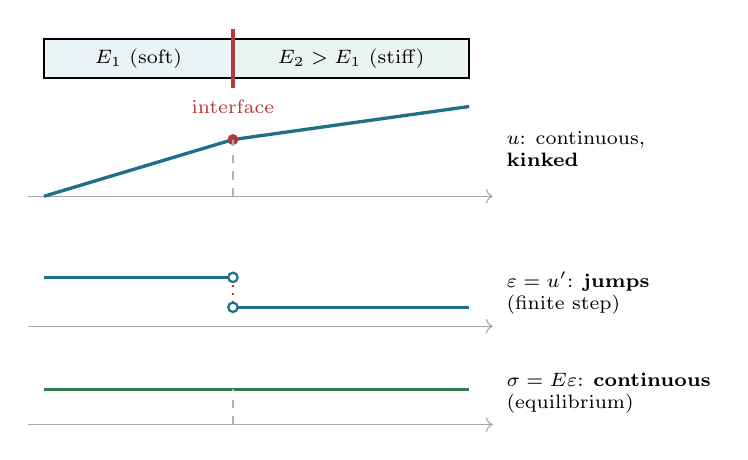
\begin{tikzpicture}[scale=1.0, every node/.style={font=\small}]
% bimaterial bar
\begin{scope}[shift={(0,2.55)}]
  \fill[IntBack] (0,0) rectangle (2.4,0.5);
  \fill[MEBack]  (2.4,0) rectangle (5.4,0.5);
  \draw[thick] (0,0) rectangle (5.4,0.5);
  \draw[very thick,PitFrame] (2.4,-0.12) -- (2.4,0.62);
  \node[font=\scriptsize] at (1.2,0.25) {$E_{1}$ (soft)};
  \node[font=\scriptsize] at (3.9,0.25) {$E_{2}>E_{1}$ (stiff)};
  \node[below,font=\scriptsize,PitFrame] at (2.4,-0.16) {interface};
\end{scope}
% displacement
\begin{scope}[shift={(0,1.05)}]
  \draw[->,gray!70] (-0.2,0) -- (5.7,0);
  \draw[very thick,IntFrame] (0,0) -- (2.4,0.72) -- (5.4,1.14);
  \fill[PitFrame] (2.4,0.72) circle (2pt);
  \draw[dashed,gray!60] (2.4,0) -- (2.4,0.72);
  \node[right,font=\scriptsize,align=left] at (5.75,0.6) {$u$: continuous,\\ \textbf{kinked}};
\end{scope}
% strain
\begin{scope}[shift={(0,-0.6)}]
  \draw[->,gray!70] (-0.2,0) -- (5.7,0);
  \draw[very thick,IntFrame] (0,0.62) -- (2.4,0.62);
  \draw[very thick,IntFrame] (2.4,0.24) -- (5.4,0.24);
  \draw[dotted,thick,PitFrame] (2.4,0.62) -- (2.4,0.24);
  \draw[IntFrame,fill=white,thick] (2.4,0.62) circle (1.7pt);
  \draw[IntFrame,fill=white,thick] (2.4,0.24) circle (1.7pt);
  \node[right,font=\scriptsize,align=left] at (5.75,0.42) {$\eps=u'$: \textbf{jumps}\\ (finite step)};
\end{scope}
% stress
\begin{scope}[shift={(0,-1.85)}]
  \draw[->,gray!70] (-0.2,0) -- (5.7,0);
  \draw[very thick,MEFrame] (0,0.45) -- (5.4,0.45);
  \draw[dashed,gray!60] (2.4,0) -- (2.4,0.45);
  \node[right,font=\scriptsize,align=left] at (5.75,0.4) {$\sigma=E\eps$: \textbf{continuous}\\ (equilibrium)};
\end{scope}
\end{tikzpicture}
\caption{Bimaterial bar: $\sigma$ continuous (equilibrium), so $\eps=u'$ jumps and $u$ kinks. \textbf{Put a node at the interface} --- a linear element cannot bend inside itself.}
\label{fig:bimaterial}
\end{figure}

\noindent
Same for any abrupt change --- a step in area, a point load, a change in
distributed load, the edge of a contact patch. \emph{Put a node there.}

% ------------------------------------------------------------------
\subsection{Bars versus beams: the rule shifts up one rung}

\begin{figure}[htbp]
\centering
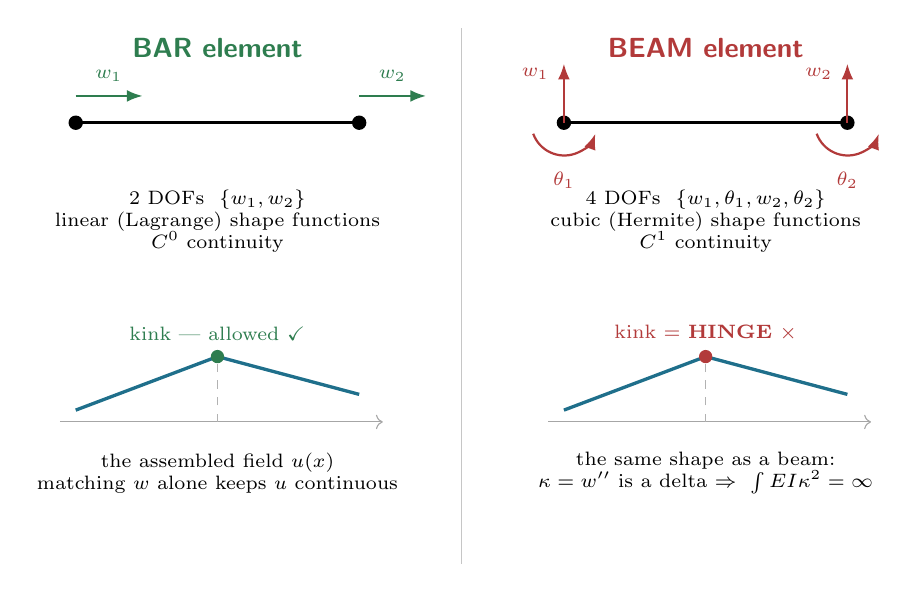
\begin{tikzpicture}[scale=1.0, every node/.style={font=\small}]
\node[font=\bfseries\sffamily,MEFrame]  at (2.2,3.05) {BAR element};
\node[font=\bfseries\sffamily,PitFrame] at (8.4,3.05) {BEAM element};
\draw[gray!45] (5.3,-3.5) -- (5.3,3.3);

% ---------------- bar: the element ----------------
\begin{scope}[shift={(0.4,2.1)}]
  \draw[very thick] (0,0) -- (3.6,0);
  \fill (0,0) circle (2.6pt); \fill (3.6,0) circle (2.6pt);
  \draw[-{Latex[length=2mm]},MEFrame,thick] (0,0.34) -- (0.85,0.34);
  \draw[-{Latex[length=2mm]},MEFrame,thick] (3.6,0.34) -- (4.45,0.34);
  \node[MEFrame,font=\scriptsize,above] at (0.42,0.4) {$w_{1}$};
  \node[MEFrame,font=\scriptsize,above] at (4.02,0.4) {$w_{2}$};
\end{scope}
\node[font=\scriptsize,align=center] at (2.2,0.85)
  {2 DOFs \ $\{w_{1},w_{2}\}$\\ linear (Lagrange) shape functions\\ $C^{0}$ continuity};

% ---------------- bar: assembled field ----------------
\begin{scope}[shift={(0.4,-1.55)}]
  \draw[->,gray!70] (-0.2,-0.15) -- (3.9,-0.15);
  \draw[very thick,IntFrame] (0,0) -- (1.8,0.68) -- (3.6,0.2);
  \fill[MEFrame] (1.8,0.68) circle (2.4pt);
  \draw[dashed,gray!60] (1.8,-0.15) -- (1.8,0.68);
  \node[above,font=\scriptsize,MEFrame] at (1.8,0.76) {kink --- allowed \cmark};
\end{scope}
\node[font=\scriptsize,align=center] at (2.2,-2.35)
  {the assembled field $u(x)$\\ matching $w$ alone keeps $u$ continuous};

% ---------------- beam: the element ----------------
\begin{scope}[shift={(6.6,2.1)}]
  \draw[very thick] (0,0) -- (3.6,0);
  \fill (0,0) circle (2.6pt); \fill (3.6,0) circle (2.6pt);
  \draw[-{Latex[length=2mm]},PitFrame,thick] (0,0) -- (0,0.75);
  \draw[-{Latex[length=2mm]},PitFrame,thick] (3.6,0) -- (3.6,0.75);
  \draw[-{Latex[length=2mm]},PitFrame,thick] (-0.39,-0.14) arc (200:340:0.42);
  \draw[-{Latex[length=2mm]},PitFrame,thick] (3.21,-0.14) arc (200:340:0.42);
  \node[PitFrame,font=\scriptsize,left]  at (-0.07,0.62) {$w_{1}$};
  \node[PitFrame,font=\scriptsize,left]  at (3.53,0.62) {$w_{2}$};
  \node[PitFrame,font=\scriptsize,below] at (0,-0.5)    {$\theta_{1}$};
  \node[PitFrame,font=\scriptsize,below] at (3.6,-0.5)  {$\theta_{2}$};
\end{scope}
\node[font=\scriptsize,align=center] at (8.4,0.85)
  {4 DOFs \ $\{w_{1},\theta_{1},w_{2},\theta_{2}\}$\\ cubic (Hermite) shape functions\\ $C^{1}$ continuity};

% ---------------- beam: assembled field ----------------
\begin{scope}[shift={(6.6,-1.55)}]
  \draw[->,gray!70] (-0.2,-0.15) -- (3.9,-0.15);
  \draw[very thick,IntFrame] (0,0) -- (1.8,0.68) -- (3.6,0.2);
  \fill[PitFrame] (1.8,0.68) circle (2.4pt);
  \draw[dashed,gray!60] (1.8,-0.15) -- (1.8,0.68);
  \node[above,font=\scriptsize,PitFrame] at (1.8,0.76) {kink $=$ \textbf{HINGE} \xmark};
\end{scope}
\node[font=\scriptsize,align=center] at (8.4,-2.35)
  {the same shape as a beam:\\ $\kappa=w''$ is a delta $\Rightarrow\ \int EI\kappa^{2}=\infty$};
\end{tikzpicture}
\caption{Bar: matching $w$ keeps $u$ continuous. Beam: the energy holds $w''$, so the \emph{slope} must match too --- else every node is a hinge.}
\label{fig:barbeam}
\end{figure}

\begin{center}\small
\renewcommand{\arraystretch}{1.25}
\begin{tabular}{@{}l l l@{}}
\toprule
 & \textbf{Bar / truss / solid / heat} & \textbf{Beam / plate / shell}\\
\midrule
field                 & $w$ = displacement          & $w$ = deflection\\
energy contains       & $w'$ \ (strain)             & $w''$ \ (curvature)\\
PDE order             & 2 \quad $-(EA\,w')'=f$      & 4 \quad $(EI\,w'')''=q$\\
space                 & $H^{1}$: $\int (w')^{2}<\infty$ & $H^{2}$: $\int (w'')^{2}<\infty$\\
must stay continuous  & $w$                         & $w$ \emph{and} $w'$\\
\textbf{kink in $w$}  & allowed \cmark              & \textbf{forbidden} \xmark \ (a hinge)\\
\textbf{jump in $w$}  & forbidden \xmark            & forbidden \xmark\\
element continuity    & $C^{0}$                     & $C^{1}$\\
nodal DOFs            & $\{w\}$                     & $\{w,\theta\}$\\
shape functions       & linear hat (Lagrange)       & cubic Hermite\\
\bottomrule
\end{tabular}
\end{center}

\medskip\noindent
\textbf{The master rule.} \emph{The highest derivative appearing in the energy
fixes the space, which fixes the continuity the elements must have, which fixes
the degrees of freedom at each node.} Everything in the table follows from the
left-hand column of its own row.

% ------------------------------------------------------------------
\subsection{When you genuinely \emph{want} a jump}

Real structures do crack, delaminate, slip, and separate. Since a conforming
$C^{0}$ space cannot represent a jump, you have to introduce one deliberately:

\begin{center}\small
\renewcommand{\arraystretch}{1.2}
\begin{tabular}{@{}ll@{}}
\toprule
\textbf{Situation} & \textbf{How the jump is admitted}\\
\midrule
crack along element boundaries & duplicate the nodes; the two faces get independent DOFs\\
crack cutting through elements & XFEM / GFEM: \emph{enrich} the basis with a discontinuous function\\
progressive separation         & cohesive-zone elements: a traction--separation law across the interface\\
contact / frictional slip      & separate meshes plus constraints (multipliers, penalty)\\
shocks, advection dominance    & discontinuous Galerkin: give up $\Vh\subset V$ on purpose\\
\bottomrule
\end{tabular}
\end{center}

\noindent
None of these arise by accident: a conforming FE model \emph{cannot} tear on its
own. That guarantee is what makes ordinary structural analysis trustworthy, and
the obstacle you must go around to model fracture.

Flip side: the FE solution is continuous with kinks at nodes, so its
\emph{stress is discontinuous across element boundaries}. The jumpy contour plot
before smoothing is $\Vh$ being honest --- and the size of those jumps measures
discretisation error, the basis of the Zienkiewicz--Zhu estimator.

% ==================================================================
\section{Summary}

\begin{intuition}[the one-page version]
\textbf{A kink breaks the slope. A jump breaks the shape.}
\begin{itemize}[leftmargin=1.4em,itemsep=3pt]
  \item Differentiating a kink gives a \textbf{step}: bounded, squares
        harmlessly, finite energy. \emph{Allowed.}
  \item Differentiating a jump gives a \textbf{delta}: unbounded, finite area
        but infinite squared area, infinite energy. \emph{Forbidden.}
  \item $V=H^{1}_{0}$ is exactly the set that admits the first and excludes the
        second --- big enough for hat functions, small enough to keep the bar
        in one piece.
  \item Every FE displacement field is kinked at every node, by construction,
        and that is fine. What element assembly enforces is only that it never
        jumps.
  \item Differentiate once more and the hat's second derivative is a delta ---
        so the hat is in $H^{1}$ but not $H^{2}$. That one fact separates
        $C^{0}$ bar elements from $C^{1}$ beam elements, and is why beam nodes
        carry rotations.
  \item Where the exact solution kinks (material interface, point load, section
        change), \textbf{put a node}.
\end{itemize}
\end{intuition}

\end{document}
